%%%%%%%%%%%%%%%%%%%%%%%%%%%%%%%%%%%%%%%%%%
% Engineering problems / LaTeX Template
%		Semester 6
%		Institut d'Optique Graduate School
%%%%%%%%%%%%%%%%%%%%%%%%%%%%%%%%%%%%%%%%%%
%	6N-IntNum-BlocRobot	/ Embedded System
%%%%%%%%%%%%%%%%%%%%%%%%%%%%%%%%%%%%%%%%%%
%
% Created by:
%	Julien VILLEMEJANE - 19/oct/2024	
%
%%%%%%%%%%%%%%%%%%%%%%%%%%%%%%%%%%%%%%%%%%
% Professional Newsletter Template
% LaTeX Template
% Version 1.0 (09/03/14)
%
% Created by:
% Bob Kerstetter (https://www.tug.org/texshowcase/) and extensively modified by:
% Vel (vel@latextemplates.com)
% 
% This template has been downloaded from:
% http://www.LaTeXTemplates.com
%
% License:
% CC BY-NC-SA 3.0 (http://creativecommons.org/licenses/by-nc-sa/3.0/)
%
%%%%%%%%%%%%%%%%%%%%%%%%%%%%%%%%%%%%%%%%%

\documentclass[a4paper,11pt,titlepage]{article} % The default font size is 10pt; 11pt and 12pt are alternatives

%%%%%%%%%%%%%%%%%%%%%%%%%%%%%%%%%%%%%%%%%%%%%%%%%%%%%%%%%%%%%%%%%%%%%%%%%%%%%%%%%%%%%%%%%%%%%%%%%%%%%%%%%%%%%%%%%%%%%%%%%%%%%%%%%%%%%%%%%%%%%%%%%%%%%%%%%%%%%%%%%%%%%%%%%%%%%%%%%%%%%%%%%%%%%%%%%%%%%%%%%%%%%%%%%%%%%%%%%%%%%%%%%%%%%%%%%%%%%%%%%%%%%%%%%%%%
\usepackage{opto_elec_villemejane}
\usetikzlibrary{positioning}

%%%%%%%%%%%%%%%%%%%%%%%%%%%%%%%%%%%%%%%%%%%%%%%%
%%%%%%%%%%%%%%%%%%%%%%%%%%%%%%%%%%%%%%%%%%%%%%%%
\begin{document}



% Page de garde
\begin{titlepage}

\begin{center}
	\begin{minipage}{2.5cm}
	\begin{center}
		
\includegraphics[width=8cm]{images/Logo-LEnsE.png}
	\end{center}
\end{minipage}\hfill
\begin{minipage}{10cm}
	\begin{center}
	\textbf{Institut d'Optique Graduate School }\\[0.1cm]
    \textbf{Interfaçage Numérique}


	\end{center}
\end{minipage}\hfill


\vspace{4cm}


{\huge \bfseries \textsc{Interfaçage Numérique}} \\[0.5cm]
{\large \bfseries Travaux Pratiques} \\[0.2cm]
Semestre 6

\vspace{2cm}
% Title
\rule{\linewidth}{0.3mm} \\[0.4cm]
{ \huge \bfseries\color{violet_iogs} Banc de mesure de rayonnement \\[0.4cm] }
\rule{\linewidth}{0.3mm} \\[1cm]

4 séances

\bigskip

\begin{center}
	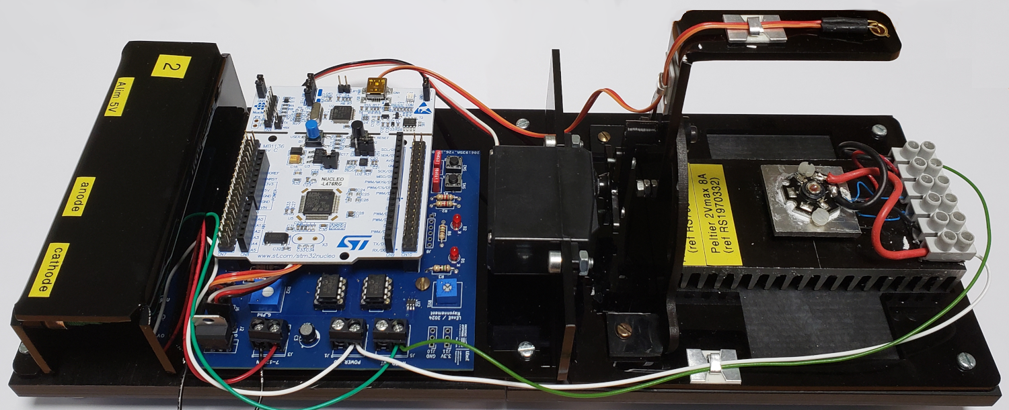
\includegraphics[width=0.7\textwidth]{images/rayonnement.png}
\end{center}

\vfill

\textit{Ce sujet est disponible au format électronique sur le site du LEnsE - https://lense.institutoptique.fr/ dans la rubrique Année / Première Année / Interfaçage Numérique S6 / Bloc 1 Systèmes embarqués / Banc de mesure de rayonnement lumineux.}

% Bottom of the page
%{\textbf{\large {Année universitaire} 2024-2025}}

\end{center}
\end{titlepage}

\newpage
\strut % empty page


%%%%%%%%%%%%%%%%%%%%%%%%%%%%%%%%%%%%%%%%%%%%%%%%
%%%%%%%%%%%%%    Intro
\newpage
\pagestyle{empty}

\begin{minipage}[c]{.25\linewidth}
	
\includegraphics[width=5cm]{images/Logo-LEnsE.png}
\end{minipage} \hfill
\begin{minipage}[c]{.4\linewidth}

\begin{center}
\vspace{0.3cm}
{\Large \textsc{Interfaçage Numérique}}

\medskip

6N-047-SCI \qquad \textbf{\large Bloc Rayonnement}

\end{center}
\end{minipage}\hfill

\vspace{0.5cm}

\noindent \rule{\linewidth}{1pt}

{\noindent\Large  \rule[-7pt]{0pt}{30pt} \textbf{Banc de mesure de rayonnement}}

\noindent \rule{\linewidth}{1pt}

\bigskip 

%%%%%%%%%%%%%%%%%%%%%%%%%%%%%%%%%%%%%%%%%%%%%%%%
%%%%%%%%%%%%%    A A V

{\large À l'issue des séances de TP concernant le \textbf{bloc d'acquisition d'un diagramme de rayonnement}, les étudiant$\cdot$es seront capables de :}

\medskip

\begin{itemize}
	\item Développer et mettre en \oe{}uvre une \textbf{solution d'électronique embarquée} pour \textbf{acquérir des données analogiques} et commander un élément mobile.
	\item Mettre en \oe{}uvre un \textbf{protocole simple de communication} entre un ordinateur et un microcontrôleur pour transmettre des commandes et lire des données
	\item Optimiser une \textbf{interface informatique} de pilotage et d'affichage de données
\end{itemize}

\noindent \rule{\linewidth}{1pt}


%%%%%%%%%%%%%%%%%%%%%%%%%%%%%%%%%%%%%%%%%%%%%%%%
%%%%%%%%%%%%%    Objectifs

\section{Objectifs du mini-projet}

L'objectif principal de ce mini-projet est d'\textbf{automatiser un banc de mesure de rayonnement lumineux} à l'aide d'un ordinateur et d'une interface en Python. Le matériel est piloté par une carte à microcontroleur à laquelle il faudra envoyer des commandes selon un protocole série.

\medskip

Un diagramme de rayonnement lumineux est la \textbf{représentation graphique} de la \textbf{distribution angulaire} d'une grandeur caractérisant le rayonnement d'une source lumineuse.

\begin{center}
	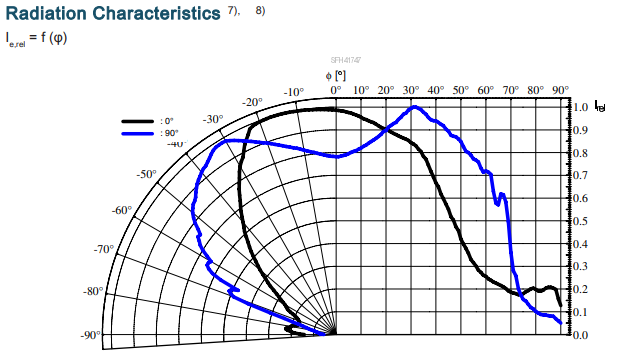
\includegraphics[width=0.7\textwidth]{images/osram_sfh41747.png}
	
	Exemple de diagramme de rayonnement d'une LED OSRAM SFH 41747 (documentation technique)
\end{center}


\medskip

Vous aurez à votre disposition une \textbf{maquette} permettant la mise en mouvement d'un système de photodétection autour d'une source de puissance à LED. Cette maquette est pilotée par une carte Nucléo (contenant un microcontroleur).


%%%%%%%%%%%%%%%%%%%%%%%%%%%%%%%%%%%%%%%%%%%%%%%%
%%%%%%%%%%%%%    Déroulement

\section{Déroulement du bloc}

\textit{La liste des étapes à suivre pour la réalisation du programme embarqué de la plateforme de rayonnement lumineux est donnée à titre indicatif. L'ordre et le choix des différentes étapes sont laissés à l'appréciation des différents binômes.}

\textit{Afin de faciliter la réutilisation des codes, il pourra être intéressant de définir des fonctions pour le pilotage des différents éléments.}

\subsection{Séance 1 / MBED et Nucléo-STM32 (sans maquette !!)}

\textit{Le sujet de cette séance est fourni dans un document annexe, disponible aussi sur le site du LEnsE - https://lense.institutoptique.fr/ dans la rubrique Année / Première Année / Interfaçage Numérique S6 / Bloc 1 Systèmes embarqués / Intro MBED et STM32.}

	\begin{description}
		\item[Etape 0 - 30 min] Créer un compte MBED et tester un premier programme
		\item[Etape 1 - 45 min] Piloter des sorties numériques - LED
		\item[Etape 2 - 45 min] Acquérir des données numériques - Bouton-poussoirs
		\item[Etape 3 - 45 min] Mettre en \oe{}uvre des interruptions sur des événements externes
		\item[Etape 4 - 45 min] Utiliser des sorties modulées en largeur d'impulsion (PWM) - LEDs
		\item[Etape 5 - 60 min] Acquérir des données analogiques - Potentiomètre
	\end{description}	

\subsection{Séance 2 / Prise en main de la maquette et automatisation de la mesure}

	\begin{description}
		\item[Etape 6 - 60 min] Piloter l'intensité des LEDs de la maquette
		\item[Etape 7 - 60 min] Piloter le servomoteur de la maquette
		\item[Etape 8 - 90 min] Définir et tester une première structure de code permettant de piloter le servomoteur en faisant une acquisition de la luminosité à pas régulier
		\item[Etape 9 - 60 min] Récupérer les données à l'aide d'une liaison Série
	\end{description}
	
\subsection{Séance 3 / Mise en place d'un protocole de communication}

	\begin{description}
		\item[Etape 10 - 90 min] Mettre en place un protocole de communication basé sur une liste de commandes et intégrer à la structure du code embarqué
		\item[Etape 11 - 90 min] Utiliser la bibliothèque pySerial en Python pour envoyer les commandes à la carte Nucléo
		\item[Etape 12 - 90 min] Tester la communication entre la carte Nucléo et le script Python pour afficher les données
	\end{description}

\medskip


\subsection{Séance 4 / Application complète}

Cette dernière séance sera consacrée à la finalisation des différents programmes : embarqué sur la carte Nucléo pour la mesure automatique et sur l'ordinateur pour le pilotage de la maquette et l'affichage des données.

Selon le temps restant, il sera possible d'intégrer les fonctions écrites en Python dans une interface graphique, dont la structure de base est fournie.


\cleardoublepage
\strut % empty page
%%%%%%%%%%%%%%%%%%%%%%%%%%%%%%%%%%%%%%%%%%%%%%%%
%%%%%%%%%%%%%    Séance 2 détaillée

\begin{minipage}[c]{.25\linewidth}
	
\includegraphics[width=4cm]{images/Logo-LEnsE.png}
\end{minipage} \hfill
\begin{minipage}[c]{.4\linewidth}

\begin{center}
\vspace{0.3cm}
{\Large \textsc{Interfaçage Numérique}}

\medskip

6N-047-SCI \qquad \textbf{\large Bloc Rayonnement}

\end{center}
\end{minipage}\hfill

\vspace{0.5cm}

\noindent \rule{\linewidth}{1pt}

{\noindent\Large \rule[-7pt]{0pt}{30pt} Séance 2 / Prise en main de la maquette et automatisation de la mesure} 

\noindent \rule{\linewidth}{1pt}


%%%%%%%%%%%%%%%%%%%%%%%%%%%%%%%%%%%%%%%%%%%%%%%%
%%%%%%%%%%%%%    Objectifs
\section{Objectifs de la séance}

Cette seconde séance est consacrée à la \textbf{prise en main de la maquette} et à l'automatisation de la mesure de l'intensité lumineuse d'une source à LED (par exemple).


%%%%%%%%%%%%%%%%%%%%%%%%%%%%%%%%%%%%%%%%%%%%%%%%
%%%%%%%%%%%%%    Maquette
\section{Description de la maquette}


\subsection{Eléments constitutifs}

La maquette est constituée :

\begin{itemize}
	\item d'une source de lumière, une LED de puissance
	\item d'une photodiode BPX65, associée à un circuit de photodétection simple
	\item d'un servomoteur, permettant de positionner le bras supportant la photodiode au dessus de la source lumineuse selon un angle donné
	\item d'une carte de contrôle
	\item d'une carte Nucléo L476RG
\end{itemize}

\begin{center}
	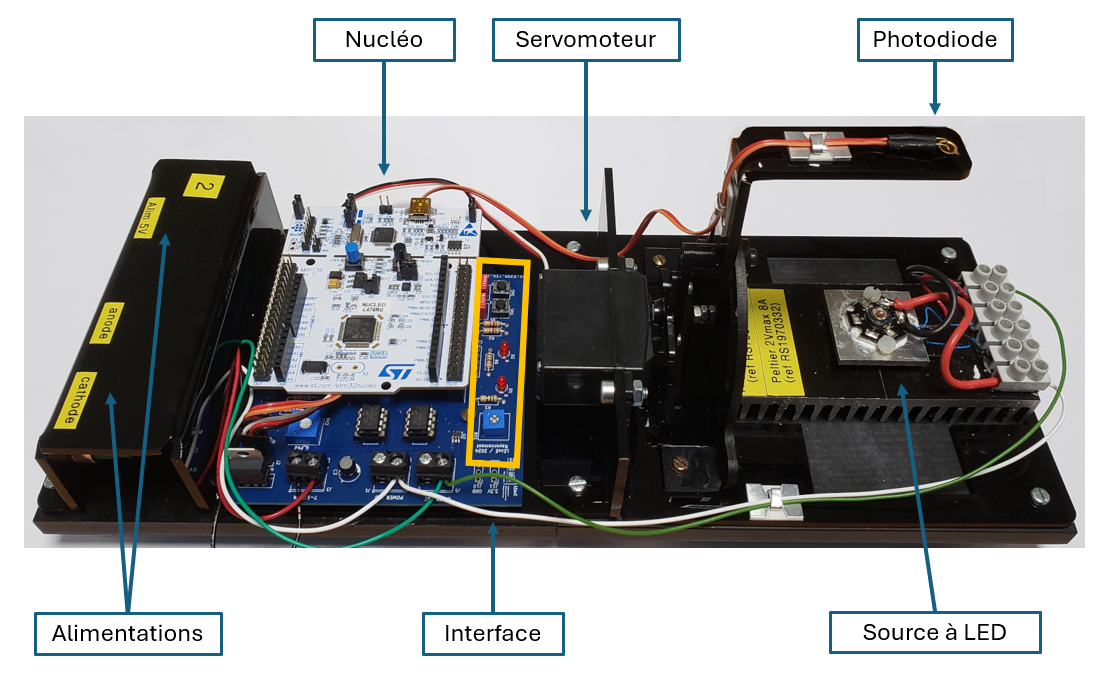
\includegraphics[width=0.9\textwidth]{images/maquette_rayon.png}
\end{center}


\subsection{Alimentation électrique}

Les bornes d'alimentation notées \textbf{Alim} $7\operatorname{V}$ permet d'alimenter le servomoteur.

Les bornes notées \textbf{anode} et \textbf{cathode} permettent d'alimenter la LED de puissance.

\noindent \rule{\linewidth}{1pt}

{\LARGE La tension maximale admissible par le servomoteur est de $7\operatorname{V}$ !}

{\Large Le courant maximal admissible par la LED de puissance est de $200\operatorname{mA}$ !}

\noindent \rule{\linewidth}{1pt}


\subsection{Brochage}

La \textbf{photodiode BPX65} est polarisée. L'\textbf{anode} est représentée par un ergot. Sur cette maquette, l'\textbf{anode} est reliée par un fil \textbf{ORANGE}, la \textbf{cathode} par un file \textbf{ROUGE}.

Le servomoteur est standard. Sa connectique est constituée de 3 broches : BLANC = signal de pilotage, ROUGE = Alimentation de 5 à 6V, NOIR = masse (GND).


\begin{center}
	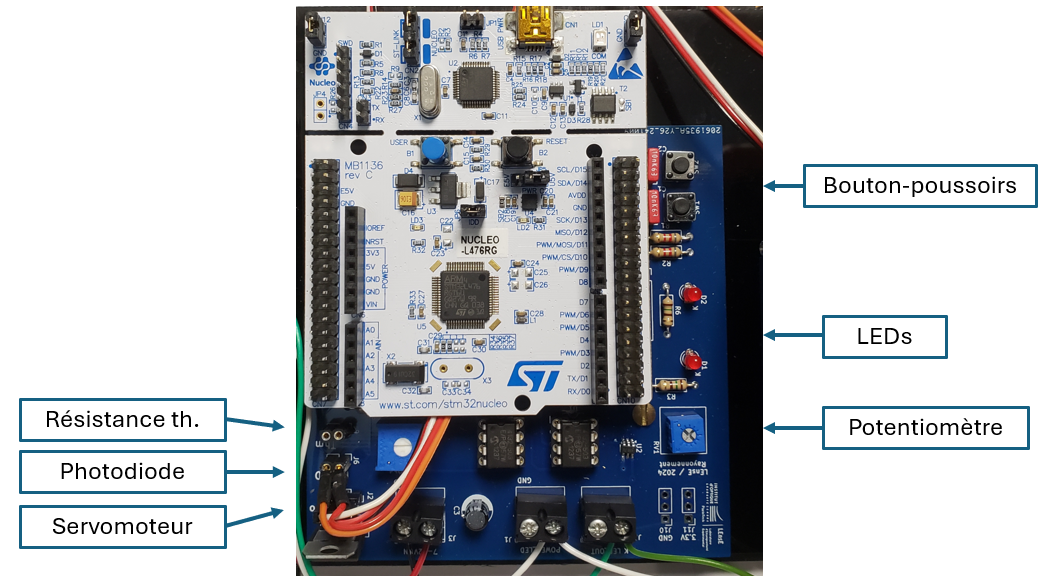
\includegraphics[width=0.7\textwidth]{images/maquette_rayon_nucleo.png}
\end{center}


\begin{center}
\begin{tabular}{|l|l|l|l|}
\hline 
Maquette & \textbf{Broche Nucléo} & Type & Description \\ 
\hline 
\textsc{LED1} & PC7 & Sortie / PWM & Led active à l'\textbf{état haut}\\ 
\textsc{LED2} & PB13 & Sortie / PWM & Led active à l'\textbf{état bas}\\ 
\hline 
\textsc{SW1} & PC6 & Entrée & Bouton-poussoir, par défaut état bas\\ 
\textsc{SW2} & PC8 & Entrée & Bouton-poussoir, par défaut état bas\\ 
\textsc{UserButton} & PC13 & Entrée & Bouton-poussoir, par défaut état haut\\
\hline 
\textsc{Servo} & PB7 & Sortie / PWM & Servomoteur - T = 20 ms\\ 
\hline 
\textsc{Potentiomètre} & PC4 & Entrée analogique & Potentiomètre RV1 \\
\hline 
\textsc{Photodiode} & PC3 & Entrée analogique & Photodiode \\
 & & & (montage simple avec R variable)\\ 
\hline 
\textsc{Résistance Thermique} & PC1 & Entrée analogique & Résistance Thermique CT10k\\ 
\hline 
\end{tabular} 
\end{center}


%%%%%%%%%%%%%%%%%%%%%%%%%%%%%%%%%%%%%%%%%%%%%%%%
%%%%%%%%%%%%%    Etape 6
\section{Etape 6 / Piloter l'intensité des LEDs de la maquette}

\Manip Réaliser un programme qui permet de modifier la luminosité des diodes LED1 et LED2 de la maquette à l'aide des deux bouton-poussoirs SW1 et SW2 (un pour augmenter, l'autre pour diminuer la luminosité). \textbf{Votre programme devra utiliser uniquement le principe d'interruption.}

\newpage
%%%%%%%%%%%%%%%%%%%%%%%%%%%%%%%%%%%%%%%%%%%%%%%%
%%%%%%%%%%%%%    Etape 7
\section{Etape 7 / Piloter le servomoteur de la maquette}

Un servomoteur est un actionneur qui réalise une rotation d'un angle calibré en fonction d'une commande externe.

\begin{center}
	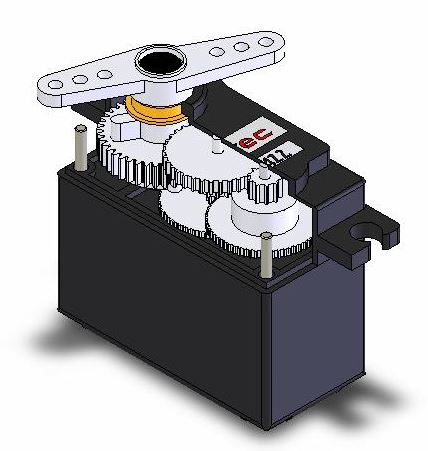
\includegraphics[width=0.3\textwidth]{images/MINE_Nucleo_servomoteur-redohm.jpg}
	
	Servomoteur - coupe interne (Crédit : redohm.fr)
\end{center}

Le pilotage d'un servomoteur se fait à l'aide d'un \textbf{signal modulé en largeur d'impulsions}. Le signal de commande est un \textbf{signal rectangulaire} (numérique) de période fixée à 20 ms. C'est ensuite la durée du temps haut qui permet de modifier l'angle de sortie du servomoteur :

\begin{center}
	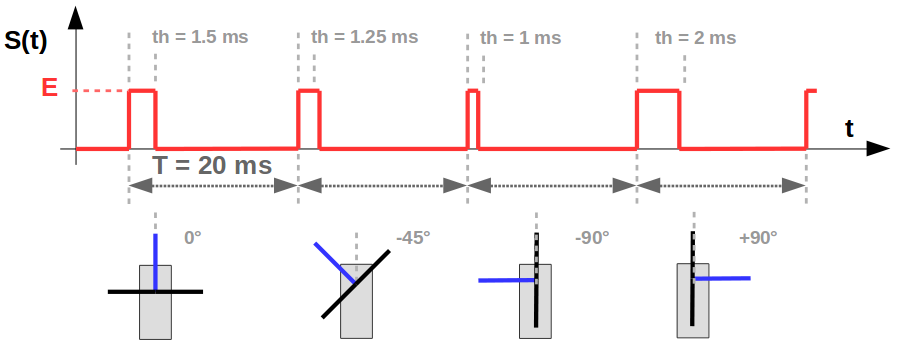
\includegraphics[width=0.8\textwidth]{images/MINE_Nucleo_servomoteur.png}
\end{center}

\subsection{Travail à réaliser}

On se propose de tester le code \textsl{pwm\_servo.cpp}. Ce fichier est disponible sur le site du LEnsE dans la rubrique \textit{Année / Première Année / Interfaçage Numérique S6 / Bloc 1 Systèmes embarqués / Exemples MBED pour STM32}.

\Manip Tester le code fourni. 

\Manip Créer une fonction permettant de positionner le servomoteur à un angle particulier. Tester votre fonction. 

\newpage
%%%%%%%%%%%%%%%%%%%%%%%%%%%%%%%%%%%%%%%%%%%%%%%%
%%%%%%%%%%%%%    Etape 8
\section{Etape 8 / Définir et tester une première structure de code}

On cherche à présent à \textbf{automatiser l'acquisition des données} de luminosité en fonction de l'angle d'observation.

\Manip Réaliser une fonction qui, à partir d'un \textbf{angle de départ}, d'un \textbf{angle d'arrivée} et d'un \textbf{pas angulaire}, permet, pour tous les angles concernés, de :

\begin{itemize}
	\item déplacer le servomoteur au prochain angle ;
	\item faire l'acquisition de la luminosité dans un tableau de données.
\end{itemize}

\textit{Le servomoteur ne réagit pas instantanément. Il est donc nécessaire d'ajouter un temps de pause entre le déplacement et l'acquisition.}

\Manip Tester votre fonction.


%%%%%%%%%%%%%%%%%%%%%%%%%%%%%%%%%%%%%%%%%%%%%%%%
%%%%%%%%%%%%%    Etape 9
\section{Etape 9 / Récupérer les données à l'aide d'une liaison Série}

\subsection{Transmission des données par liaison série}

Il est possible de transmettre des données par l'intermédiaire d'une \textbf{liaison dite Série} entre le microcontroleur et l'ordinateur.

C'est un protocole asynchrone de transfert de données point à point. Les échanges se font en \textbf{Full-Duplex} grâce à deux signaux distincts \textbf{RX} (réception) et \textbf{TX} (transmission).

\textit{Cette fonctionnalité a déjà été utilisée dans l'étape 5 pour afficher sur l'ordinateur (logiciel TeraTerm) les données converties à l'aide du convertisseur analogique numérique.}

\medskip

\Manip A partir du programme de l'étape 5 et des autres programmes que vous avez mis au point, réaliser une fonction qui permet de transmettre par la liaison série les valeurs sauvegardées dans le tableau de données précédemment acquis.

\Manip Tester votre fonction.

\subsection{Pilotage de la LED de puissance}

Le code \textsl{power\_led.cpp} fournit un ensemble d'instructions permettant de piloter l'intensité lumineuse de la LED de puissance de la maquette. Ce fichier est disponible sur le site du LEnsE dans la rubrique \textit{Année / Première Année / Interfaçage Numérique S6 / Bloc 1 Systèmes embarqués / Exemples MBED pour STM32}.

\Manip Alimenter la LED de puissance avec un courant maximal de 200mA. Elle ne s'allumera pas tant que le code n'aura pas été implémenté.

\Manip Tester alors le code fourni.

\subsection{Premier diagramme de rayonnement}


\Manip Faire l'acquisition des valeurs d'intensité lumineuse pour des angles allant de $0$ à $180^\circ{}$ par pas de $10^\circ{}$ et transmettre les données par liaison Série à l'ordinateur.


\cleardoublepage
\strut % empty page
%%%%%%%%%%%%%%%%%%%%%%%%%%%%%%%%%%%%%%%%%%%%%%%%
%%%%%%%%%%%%%    Séance 3 détaillée

\begin{minipage}[c]{.25\linewidth}
	
\includegraphics[width=4cm]{images/Logo-LEnsE.png}
\end{minipage} \hfill
\begin{minipage}[c]{.4\linewidth}

\begin{center}
\vspace{0.3cm}
{\Large \textsc{Interfaçage Numérique}}

\medskip

6N-047-SCI \qquad \textbf{\large Bloc Rayonnement}

\end{center}
\end{minipage}\hfill

\vspace{0.5cm}

\noindent \rule{\linewidth}{1pt}

{\noindent\Large \rule[-7pt]{0pt}{30pt} Séance 3 / Mise en place d'un protocole de communication} 

\noindent \rule{\linewidth}{1pt}


%%%%%%%%%%%%%%%%%%%%%%%%%%%%%%%%%%%%%%%%%%%%%%%%
%%%%%%%%%%%%%    Objectifs
\section{Objectifs de la séance}

Cette séance a pour but de mettre en place un \textbf{protocole de communication} entre la carte embarquée et l'ordinateur, d'abord à l'aide d'un moniteur série puis à l'aide d'un script en Python.

L'ordinateur, maitre de la communication, devra envoyer des commandes à la carte embarquée, qui devra les exécuter puis acquitter du bon déroulement de l'opération.


% Diagramme
\begin{center}
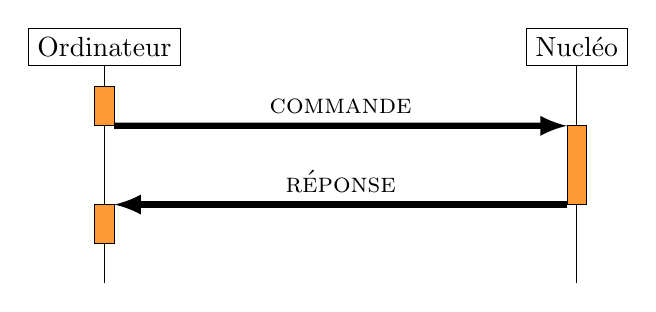
\begin{tikzpicture}

%% Locations
\def\PCToMCU{++(6,0)}
\def\MCUToPC{++(-6,0)}
\def\Lifeline{++(0,-3)}

%% Lifelines
\path (0,0)           node[draw] (PC) {Ordinateur}
      \PCToMCU node[draw] (MCU) {Nucléo};
\draw (PC) -- \Lifeline (MCU) -- \Lifeline;

%% Blocks
\path (PC)
      ++(0,-0.5) node (BeginProcess1) {} node[below right] {}
      ++(0,-0.5) node (EndProcess1)   {};
\filldraw[fill=orange!80] (BeginProcess1.east) rectangle (EndProcess1.west);

\path (MCU)
      ++(0,-1) node (BeginProcess2) {} node[below right] {}
      ++(0,-1) node (EndProcess2)   {};
\filldraw[fill=orange!80] (BeginProcess2.west) rectangle (EndProcess2.east);

\path (PC)
      ++(0,-2) node (BeginProcess3) {} node[below right] {}
      ++(0,-0.5) node (EndProcess3)   {};
\filldraw[fill=orange!80] (BeginProcess3.east) rectangle (EndProcess3.west);

%% Calls
\draw[->, line width=0.8mm, >=latex] (EndProcess1.east) -- node[above] {\textsc{commande}} (BeginProcess2.west);
\draw[->, line width=0.8mm, >=latex] (EndProcess2.west) -- node[above] {\textsc{réponse}} (BeginProcess3.east);

\end{tikzpicture}
\end{center}

\textit{Un exemple de code pour la transmission des commandes A et D, à analyser et à tester, est fourni.}

%%%%%%%%%%%%%%%%%%%%%%%%%%%%%%%%%%%%%%%%%%%%%%%%
%%%%%%%%%%%%%    Objectifs
\section{Protocole de communication}

Un \textbf{protocole de communication} est un ensemble de règles, de conventions et de formats définis pour permettre l'échange d'informations entre différents systèmes. Il détermine comment les données sont structurées, envoyées, reçues et interprétées par les parties communicantes.

\medskip

Il est important lorsqu'on souhaite \textbf{construire un protocole de communication} de :

\begin{itemize}
	\item \textbf{choisir un protocole de bas niveau} pour la transmission des commandes et des réponses
	\item définir la \textbf{structure des commandes}
	\item planifier la \textbf{liste des commandes}
	\item coder la récupération des données sur la carte Nucléo (et tester avec un moniteur Série)
	\item coder l'envoi des commandes sur le PC (en Python par exemple)
\end{itemize}


\subsection{Choix du protocole de bas niveau}

Nous utiliserons dans le cas de notre application la \textbf{liaison Série} (ou RS232) qui nous a déjà servi à afficher des données depuis la carte Nucléo.

\subsection{Structure des commandes}

Chaque commande doit avoir un \textbf{format bien défini} pour que le microcontroleur puisse la comprendre et la traiter.

\begin{center}
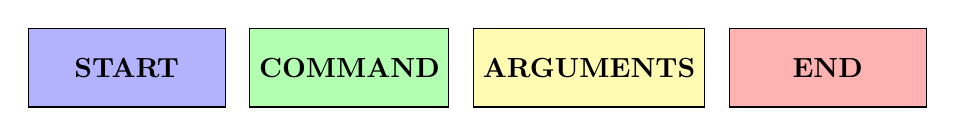
\begin{tikzpicture}[font=\sffamily]

%% Styles des blocs
\tikzstyle{block} = [rectangle, draw, minimum width=2.5cm, minimum height=1.0cm, align=center, font=\bfseries]

%% Blocs
\node[block, fill=blue!30] (start) {START};
\node[block, fill=green!30, right=0.3cm of start] (command) {COMMAND};
\node[block, fill=yellow!30, right=0.3cm of command] (arguments) {ARGUMENTS};
\node[block, fill=red!30, right=0.3cm of arguments] (end) {END};

\end{tikzpicture}
\end{center}

La liaison Série étant asynchrone, il est indispensable de prévoir dans le protocole des \textbf{caractères de début et de fin} de chaines de commande et de réponse.

\subsubsection{Commande}

Par exemple, on pourra se baser sur la structure suivante pour le cas d'une commande (entre le PC et le microcontroleur) :

\begin{center}
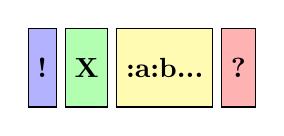
\begin{tikzpicture}[font=\sffamily]

%% Styles des blocs
\tikzstyle{block} = [rectangle, draw, minimum height=1.0cm, align=center, font=\bfseries]

%% Blocs
\node[block, fill=blue!30] (start) {!};
\node[block, fill=green!30, right=0.1cm of start] (command) {X};
\node[block, fill=yellow!30, right=0.1cm of command] (arguments) {:a:b...};
\node[block, fill=red!30, right=0.1cm of arguments] (end) {?};

\end{tikzpicture}
\end{center}

\textit{Les arguments sont facultatifs, selon les commandes.}

\subsubsection{Réponse}

Par exemple, on pourra se baser sur la structure suivante pour le cas d'une réponse (entre le PC et le microcontroleur) :

\begin{center}
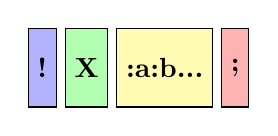
\begin{tikzpicture}[font=\sffamily]

%% Styles des blocs
\tikzstyle{block} = [rectangle, draw, minimum height=1.0cm, align=center, font=\bfseries]

%% Blocs
\node[block, fill=blue!30] (start) {!};
\node[block, fill=green!30, right=0.1cm of start] (command) {X};
\node[block, fill=yellow!30, right=0.1cm of command] (arguments) {:a:b...};
\node[block, fill=red!30, right=0.1cm of arguments] (end) {;};

\end{tikzpicture}
\end{center}

\textit{Les arguments sont facultatifs, selon les commandes.}


\subsection{Liste des commandes}

\begin{center}

\begin{tabular}{|l|l|l|}
\hline 
\textbf{Commande PC} & Description & \textbf{Réponse Nucléo} \\ 
\hline 
\textsc{!T?} & Test de la transmission & \textsc{!T;} \\ 
\hline 
\textsc{!A:value?} & Transmission de l'angle de départ souhaité pour le diagramme & \textsc{!A:value;} \\ 
 &  valeur entière en degré &  \\
 & \textit{Si angle non compris entre -90 et 90} & \textsc{value}$ = -100$ \\ 
\hline 
\textsc{!B:value?} & Transmission de l'angle final souhaité pour le diagramme & \textsc{!B:value;} \\ 
 &  valeur entière en degré &  \\ 
 & \textit{Si angle non compris entre -90 et 90} & \textsc{value}$ = -100$ \\
\hline 
\textsc{!C:value?} & Transmission du pas angulaire souhaité pour le diagramme & \textsc{!C:value;} \\ 
 &  valeur entière en degré &  \\ 
 & \textit{Si angle non compris entre -90 et 90} & \textsc{value}$ = -100$ \\
\hline 
\textsc{!S?} & Lancement de l'acquisition & \textsc{!S:nb;} \\ 
 &  nb est le nombre d'échantillons qui seront acquis par la carte &  \\ 
 & \textit{Si les angles fournis sont non compatibles} & \textsc{nb}$ = 0$ \\
\hline 
\textsc{!E?} & Test de fin de l'acquisition & \textsc{!E:Y/N;} \\
 &  (Y)es or (N)o &  \\  
\hline 
\textsc{!D:index?} & Demande de récupération d'une donnée & \textsc{!D:index:value;} \\
 &  index correspond au numéro de l'échantillon souhaité &  \\  
 &  value correspond à la valeur de l'échantillon souhaité &  \\  
\hline 
\end{tabular} 

\end{center}

%%%%%%%%%%%%%%%%%%%%%%%%%%%%%%%%%%%%%%%%%%%%%%%%
%%%%%%%%%%%%%    Etape 10
\section{Etape 10 / Mettre en place un protocole de communication basé sur une liste de commandes}

\subsection{Envoi et réception de messages simples}

Avant de se lancer dans la mise en place du protocole complet, nous vous proposons de tester l'exemple donné dans le fichier \textsl{test\_comm\_led.cpp}.

\Manip Tester le code fourni. 

\Quest A quel moment est appelée la fonction \textsl{ISR\_my\_pc\_reception()} ? A quoi sert-elle ?


\subsection{Structure de base}

On se propose de tester le code \textsl{test\_version\_a\_d.cpp}. Ce fichier est disponible sur le site du LEnsE dans la rubrique \textit{Année / Première Année / Interfaçage Numérique S6 / Banc de mesure de rayonnement lumineux / Exemples de Codes}.

\Manip Compiler ce code et le téléverser sur la carte Nucléo.

\Quest A quoi sert la fonction \textsl{is\_angle\_ok()} ?

\Manip Ouvrir le logiciel TeraTerm et envoyer la commande suivante : \textsc{!A:10?}.

\Quest Que renvoie la carte Nucléo ? Expliquer les fonctions \textsl{ISR\_my\_pc\_reception()} (vis-à-vis du choix de la structure d'une commande) et la boucle infinie. On s'intéressera notamment aux changements de valeur des variables \textsl{string\_complete} et \textsl{input\_cnt}.

\Quest Que se passe-t-il lorsqu'on transmet une mauvaise valeur (soit avec la commande A, soit avec la commande D) ?

\Quest Faire un algorigramme du code.

\subsection{Ajout des autres commandes}

On souhaite à présent compléter ce code pour pouvoir traiter l'ensemble des commandes mentionnées dans la section précédente (T, A, B, C, S, E, D).

\Manip Compléter le code précédent et le tester.

\Quest A quel moment doit-on utiliser la \textbf{fonction d'acquisition} réalisée à l'étape 8 ? D'autres commandes sont-elles acceptables lors de l'acquisition ? Comment bloquer l'exécution des autres commandes ?

\Manip Mettre en place ce blocage.

\Quest A quel moment doit-on utiliser la \textbf{fonction de transmission} des données réalisée à l'étape 9 ?


\subsection{Test complet}

\Quest Quelle est la suite de commandes à transmettre à la carte Nucléo pour permettre l'acquisition de données pour des angles allant de $-40\deg{}$ à $+60\deg{}$ par pas de $10\deg{}$ et la récupération des données sur le moniteur Série ?

\Quest Tracer le diagramme de séquence associé à ces échanges de commandes et de réponses entre le PC et la carte Nucléo.

\Manip Tester l'acquisition de cette série de données.

\newpage
%%%%%%%%%%%%%%%%%%%%%%%%%%%%%%%%%%%%%%%%%%%%%%%%
%%%%%%%%%%%%%    Etape 11
\section{Etape 11 / Utiliser la bibliothèque pySerial en Python pour envoyer les commandes à la carte Nucléo}


\begin{mdframed}[style=sidebar,frametitle={}]
\large
\textbf{ATTENTION} / Lors de l'utilisation d'un script Python nécessitant l'accès à la liaison Série, le logiciel \textbf{TeraTerm} doit être \textbf{fermé}.
\end{mdframed}


\medskip

On se propose à présent d'utiliser un script en langage Python pour pouvoir transmettre les commandes et recevoir les données sur l'ordinateur. Nous utiliserons la bibliothèques \textbf{pySerial} (à installer par la commande \textsl{pip install pyserial} dans une console ou un prompt d'Anaconda).

\medskip

Un code de base, nommé \textsl{python\_to\_Nucleo\_via\_Serial.py}, est disponible sur le site du LEnsE dans la rubrique \textit{Année / Première Année / Interfaçage Numérique S6 / Banc de mesure de rayonnement lumineux / Exemples de Codes}.

\medskip

\Manip Exécuter ce code et tester les deux commandes pré-configurées ('a' et 'd').

\Manip A partir de cet exemple, réaliser un script qui permette de lancer l'acquisition de données pour des angles allant de $-40^\circ{}$ à $+60^\circ{}$ par pas de $10^\circ{}$ et la récupération des données acquises dans une liste en Python.

\Manip Afficher les données obtenues sur un graphique à l'aide de Matplotlib. Générer l'axe des angles.


%%%%%%%%%%%%%%%%%%%%%%%%%%%%%%%%%%%%%%%%%%%%%%%%
%%%%%%%%%%%%%    Etape 12
\section{Etape 12 / Tester la communication entre la carte Nucléo et le script Python pour afficher les données}

On souhaite enfin créer une application en console complète permettant à l'utilisateur de saisir les angles de départ et de fin, le pas angulaire et de lancer l'acquisition. Votre application devra ensuite afficher les données acquises.

Vous pourrez faire plusieurs essais avec des courants dans la LED de puissance de $50\operatorname{mA}$, $100\operatorname{mA}$ et $200\operatorname{mA}$ par exemple.


\newpage
%%%%%%%%%%%%%%%%%%%%%%%%%%%%%%%%%%%%%%%%%%%%%%%%
%%% RESSOURCES COMPLEMENTAIRES		

\newpage
% Ressources
\begin{center}
	\begin{minipage}{2.5cm}
	\begin{center}
		
\includegraphics[width=5cm]{images/Logo-LEnsE.png}
	\end{center}
\end{minipage}\hfill
\begin{minipage}{10cm}
	\begin{center}
	\textbf{Institut d'Optique Graduate School }\\[0.1cm]
    \textbf{Interfaçage Numérique}


	\end{center}
\end{minipage}\hfill


\vspace{2cm}


{\Large \bfseries \textsc{Interfaçage Numérique}} \\[0.5cm]
{\large \bfseries Travaux Pratiques} \\[0.2cm]
Semestre 6

\vspace{1cm}

% Title
\rule{\linewidth}{0.4mm} \\[0.4cm]
{ \Large \bfseries\color{violet_iogs} Ressources \\[0.4cm] }
\rule{\linewidth}{0.4mm} \\[1cm]
{\large Bloc Rayonnement}

\end{center}

\vspace{3cm}

\textbf{\large Liste des ressources}
\begin{itemize}
	\item \hyperref[doc:robot_schematic]{Schéma de la carte de la maquette de rayonnement}
	\item \hyperref[doc:robot_pcb]{PCB de la carte de la maquette de rayonnement}
\end{itemize}

\vfill

%%%%%%%%%%%%%%%%%%%%%%%%%%%%%%%%%%%%%%%%%%%%%%%%
%%%%%%%%%%%%%    Autres
\section{Autres fonctionnalités}

\begin{center}
\begin{tabular}{|l|l|l|l|}
\hline 
Maquette & \textbf{Broche Nucléo} & Type & Description \\ 
\hline 
\textsc{SPI} & & & \\ 
\textit{SCK} & PA5 & Sortie & Signal d'horloge\\
\textit{MISO} & PA6 & Entrée & Données entrantes\\
\textit{MOSI} & PA7 & Sortie & Données sortantes\\
\hline 
\textsc{Pot Num} & SPI & MCP4132 & Potentiomètre Numérique\\ 
 & & & Monté dans un pont diviseur\\ 
\textit{CS} & PB9 & Sortie & \\ 
\textit{Pot Num In} & PB0 & Entrée analogique & Sortie du pont diviseur\\ 
\hline 
\textsc{LED Puissance} & SPI & MCP4132 & Potentiomètre numérique / Contrôle\\ 
 & & & courant dans Driver BCR430-UW6\\ 
\textit{CS} & PB5 & Sortie & \\
\hline 
\end{tabular} 
\end{center}

	
\begin{lstlisting}
LL_GPIO_SetAFPin_0_7(GPIOB,  GPIO_PIN_7,  GPIO_AF1_TIM2);
\end{lstlisting}

% Ressources
\titleformat{\section}
  {\null}{}{0pt}{}


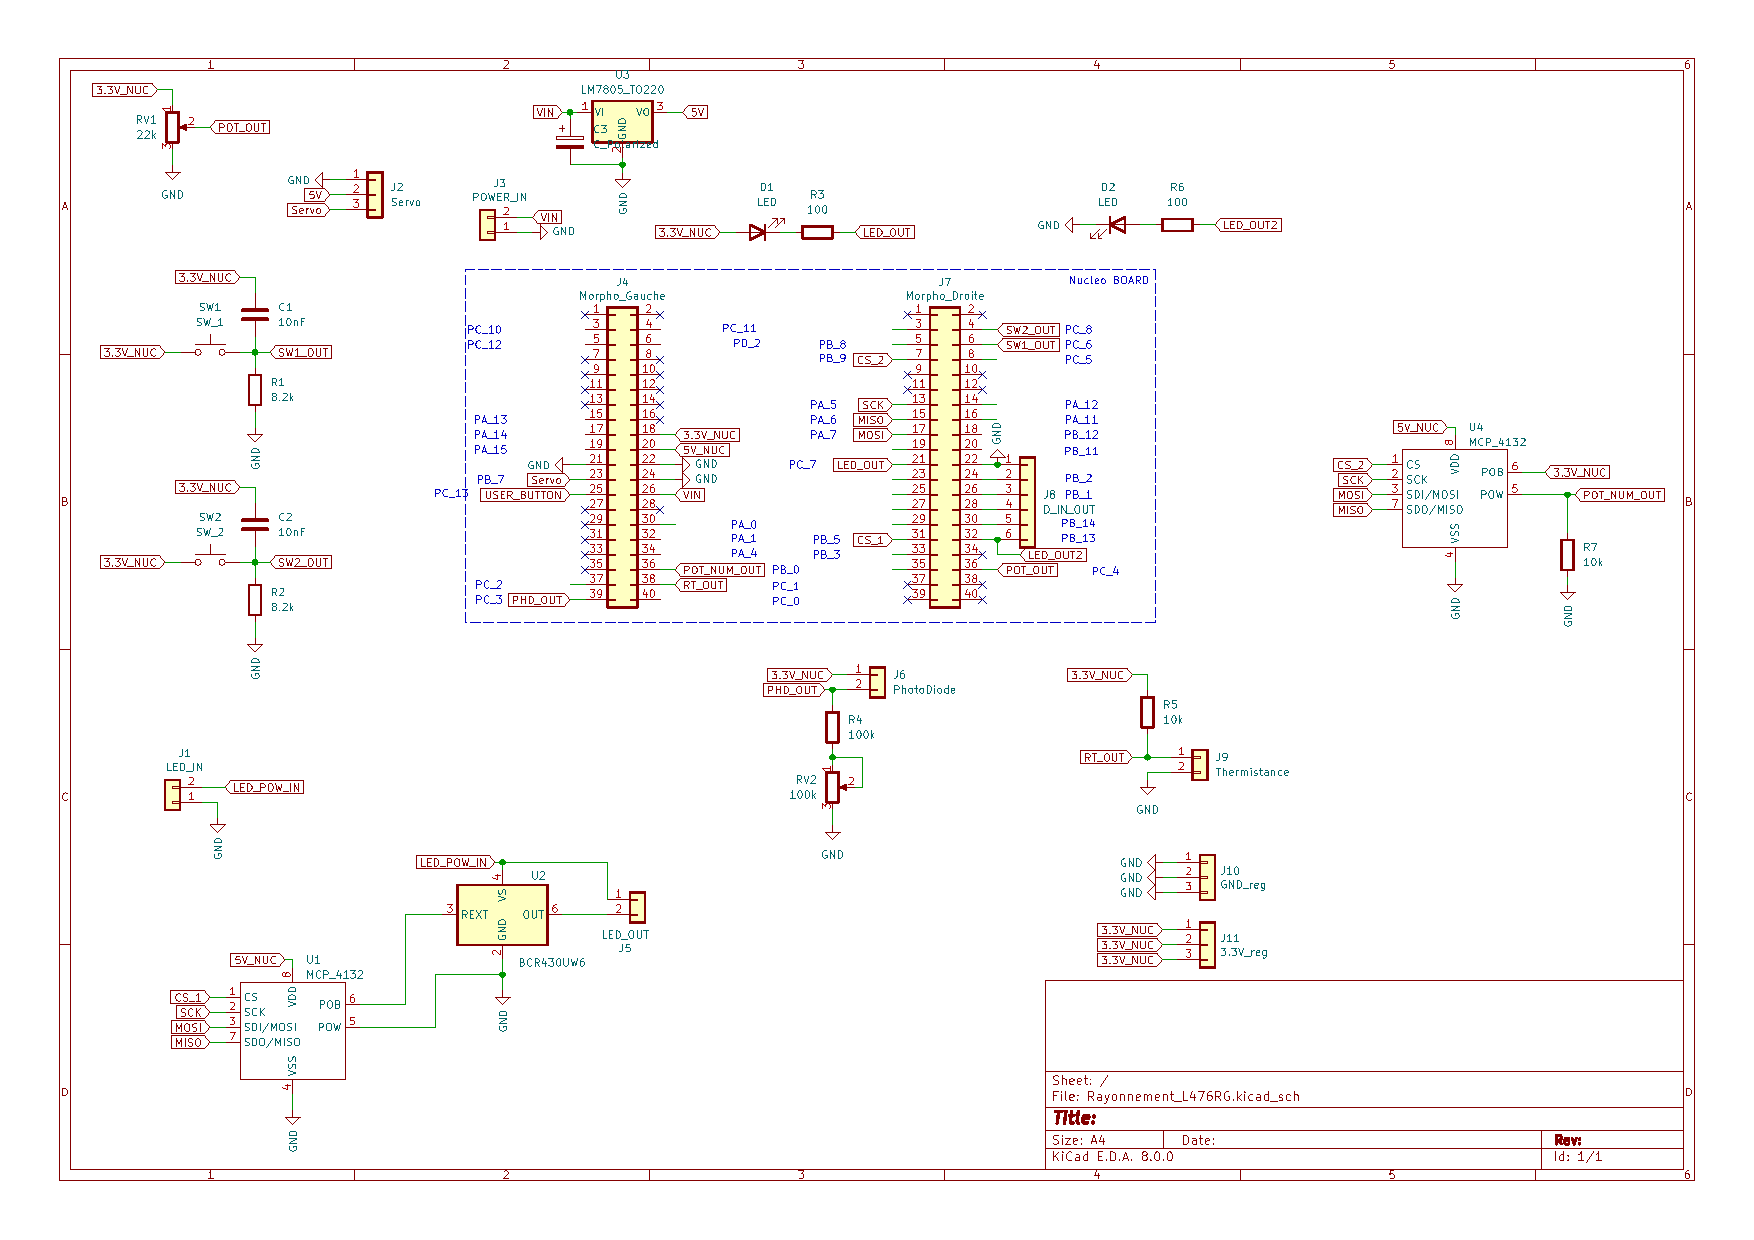
\includepdf[pages=1, landscape=true, pagecommand={\section{\texorpdfstring{\hspace{-1em}}{Schéma Carte Rayonnement}}}\label{doc:robot_schematic}]{ressources/Rayonnement_L476RG_sch.pdf}


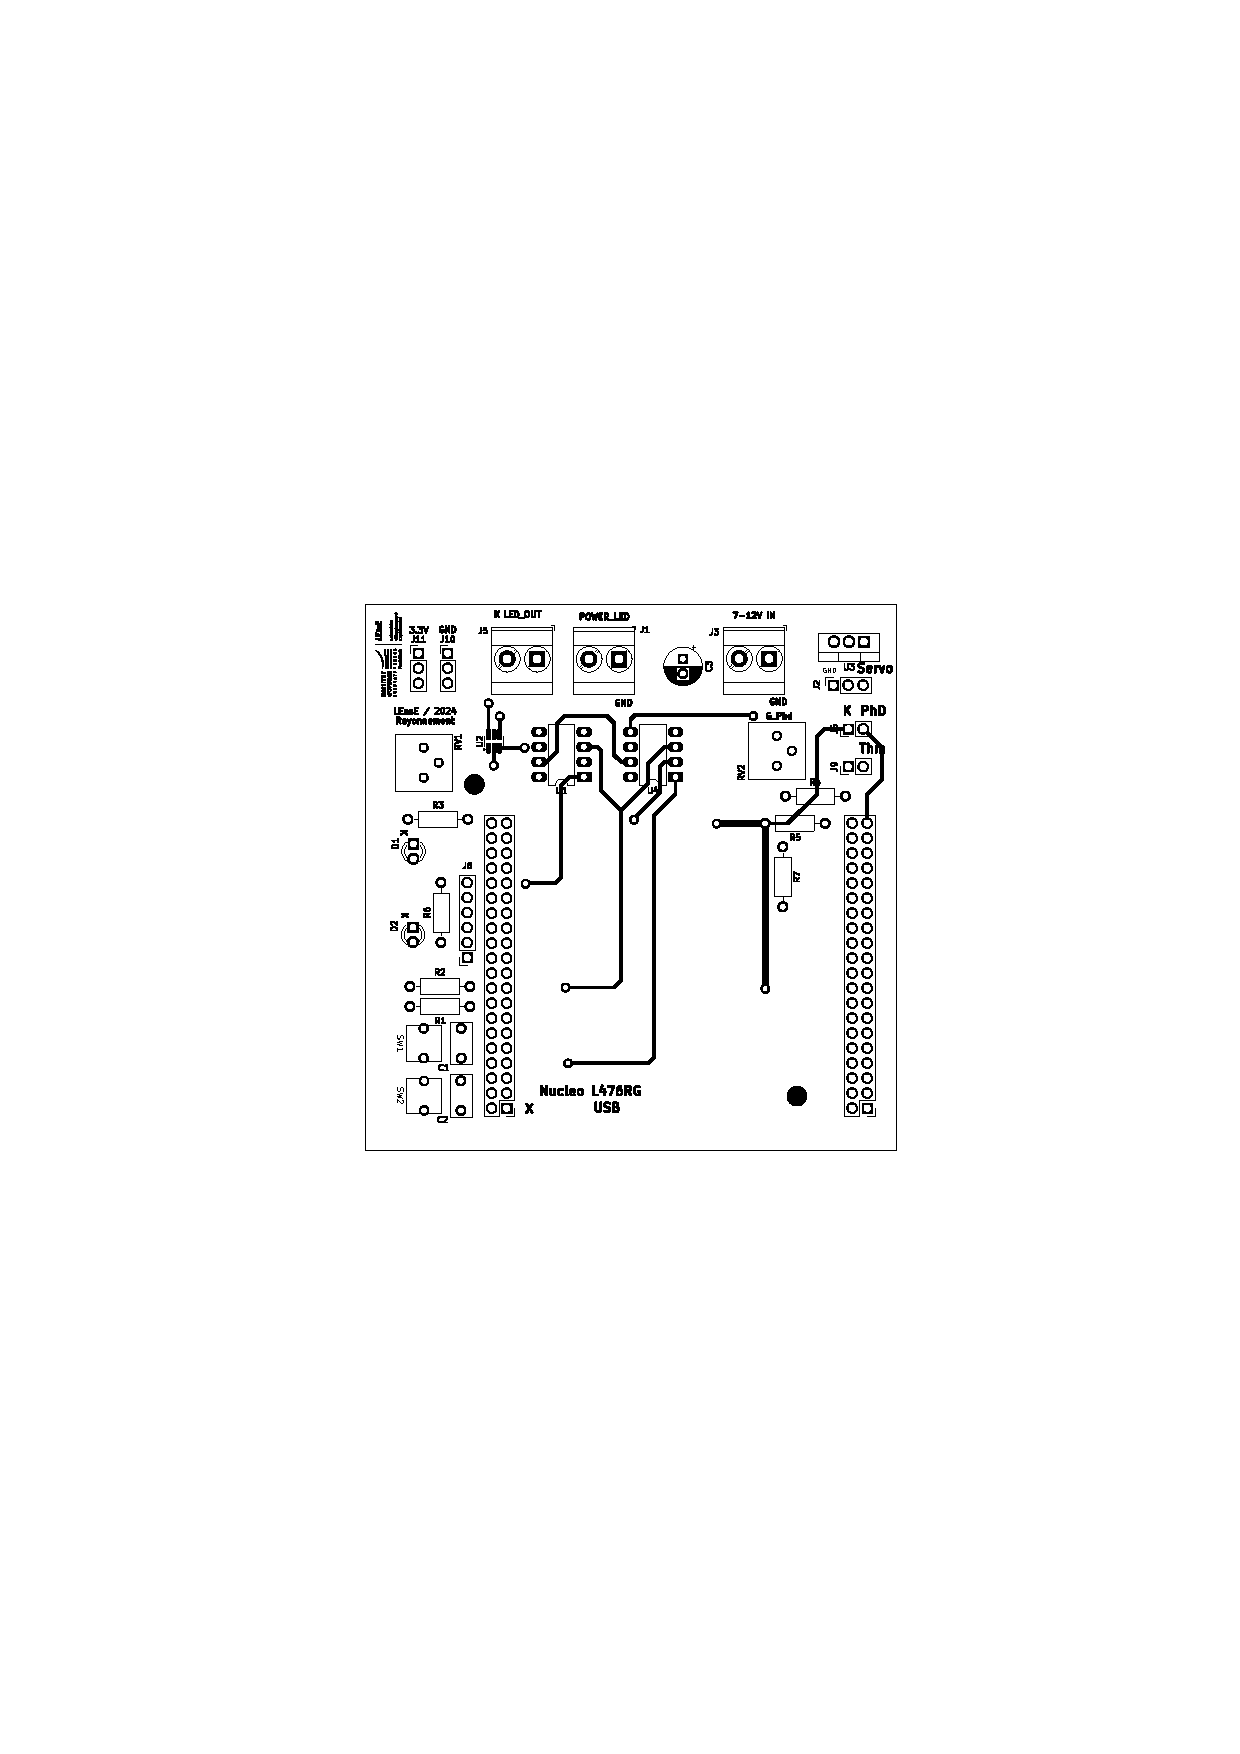
\includepdf[pages=1, pagecommand={\section{\texorpdfstring{\hspace{-1em}}{PCB Carte Rayonnement}}}\label{doc:robot_pcb}]{ressources/Rayonnement_L476RG_pcb.pdf}

\end{document}


